% !TEX root = ../main.tex

\chapter{Experiments}
\label{chapter:Experiments}
The goal of our experimental evaluation is to understand how the two main ideas of our algorithm contribute to its perforance in one observation, obscure goal 
POMDPs, namely the weak inductive bias as developed in \ref{COD_AC} and the inference time planning developed in \ref{inference_time_planning}. 
To do this, we first analyze our weak inductive bias against a proposed method using a recurrent architecture. 
We directly compare our results on the benchmark they provided. Second, we evaluate the perforance difference between pure imitation learning and reinforcement 
learning with expert demonstrations on the reach environment from the Meta-World benchmark. Here we compare our inference time planning against two state of 
the arts reinforcement learning algorithms, which are pretrained using behavioural cloning. For our third experiment setup, we evaluate our approach against 
baselines on 5 tasks from the Meta-World benchmark. As one observation POMDPs are not well studied, we propose a variety of  
baselines aiming to challenge aspects we developed in our methodology.


\section{Imitation Learning}
In this section we present our findings on the natural language conditioned robot manipulation task benchmark, that was propsed by Simon Stepputtis et.al 
\cite{stepputtis2020languageconditioned}. The benchmark consists of a 7 dof simulated robot arm with a table-top setup using CoppeliaSim which allows 
for accurate dynamics simulations at an update rate of 20Hz. The task is to pick up the correct cup and pour the content into the correct bowl, using 
natural language description of the cup and bowl and an RGB picture of the scene.\\
Three differently colored cups containing a granular material which could be poured into the bowls were used. For the bowls, 20 variations of in two sizes, 
two shape types, and five colors are used.\\
Successful picking action involved lifting a grasped object stably from the table, while successful pouring was detected whenever the cup's dispersed 
content ended up in the correct bowl. A random subset of objects was placed on the table, with a constraint to prevent collisions or other artifacts. 

Figure \ref{lang_imi_expl} depicts the table-top setup and the different variations of the objects used, as well as an example task.

As stated in section \ref{LCILRM}, in this experiment only the first observation consisting of the RGB values from the picture of the scene and the 
task description is visible for the actor. With this setup we want to evaluate our positional encoding bias. The method proposed in the accompanying 
paper "Language-Conditioned Imitation Learning for Robot Manipulation Tasks" uses a recurrent policy which we will refer to as LCIL. 
As we have motivated in section \ref{COD_AC}, 
we expect our method to perform better then autoregressive or recurrent models, because we use the knowledge that we are not getting additional information 
from the environment during the unroll of the trajectory. To test this, we have used the dataset of 40000 expert demonstrations provided 
with the benchmark to train our model using only imitation learning. 

The results are depicted in table

\begin{table}
    \centering
    \caption{Example table}
    \begin{tabular}{|c|c|c|}
        \cline{2-3}
        \multicolumn{1}{c|}{} & \textbf{Active Critic} & \textbf{LCIL} \\ \hline
        \textbf{Pick} & 100 \% & 98 \% \\ \hline
        \textbf{Pour} & 99 \% & 95 \% \\ \hline
        \textbf{Combined} & 98 \% & 92 \% \\ \hline
    \end{tabular}
    \caption{Success rates of the 100 pick, pour and combined tasks. The left column depicts the results from the Active Critic algorithm (ours) in 
    imitation mode. Right is the result of the LCIL architecture.}
\end{table}

On the 100 test environments that were provided, we decreased the overall error rate by 75$ \% $. 
\begin{figure}
    \captionsetup[subfigure]{justification=Centering, labelformat=empty}
    \begin{subfigure}[t]{0.18\textwidth}
        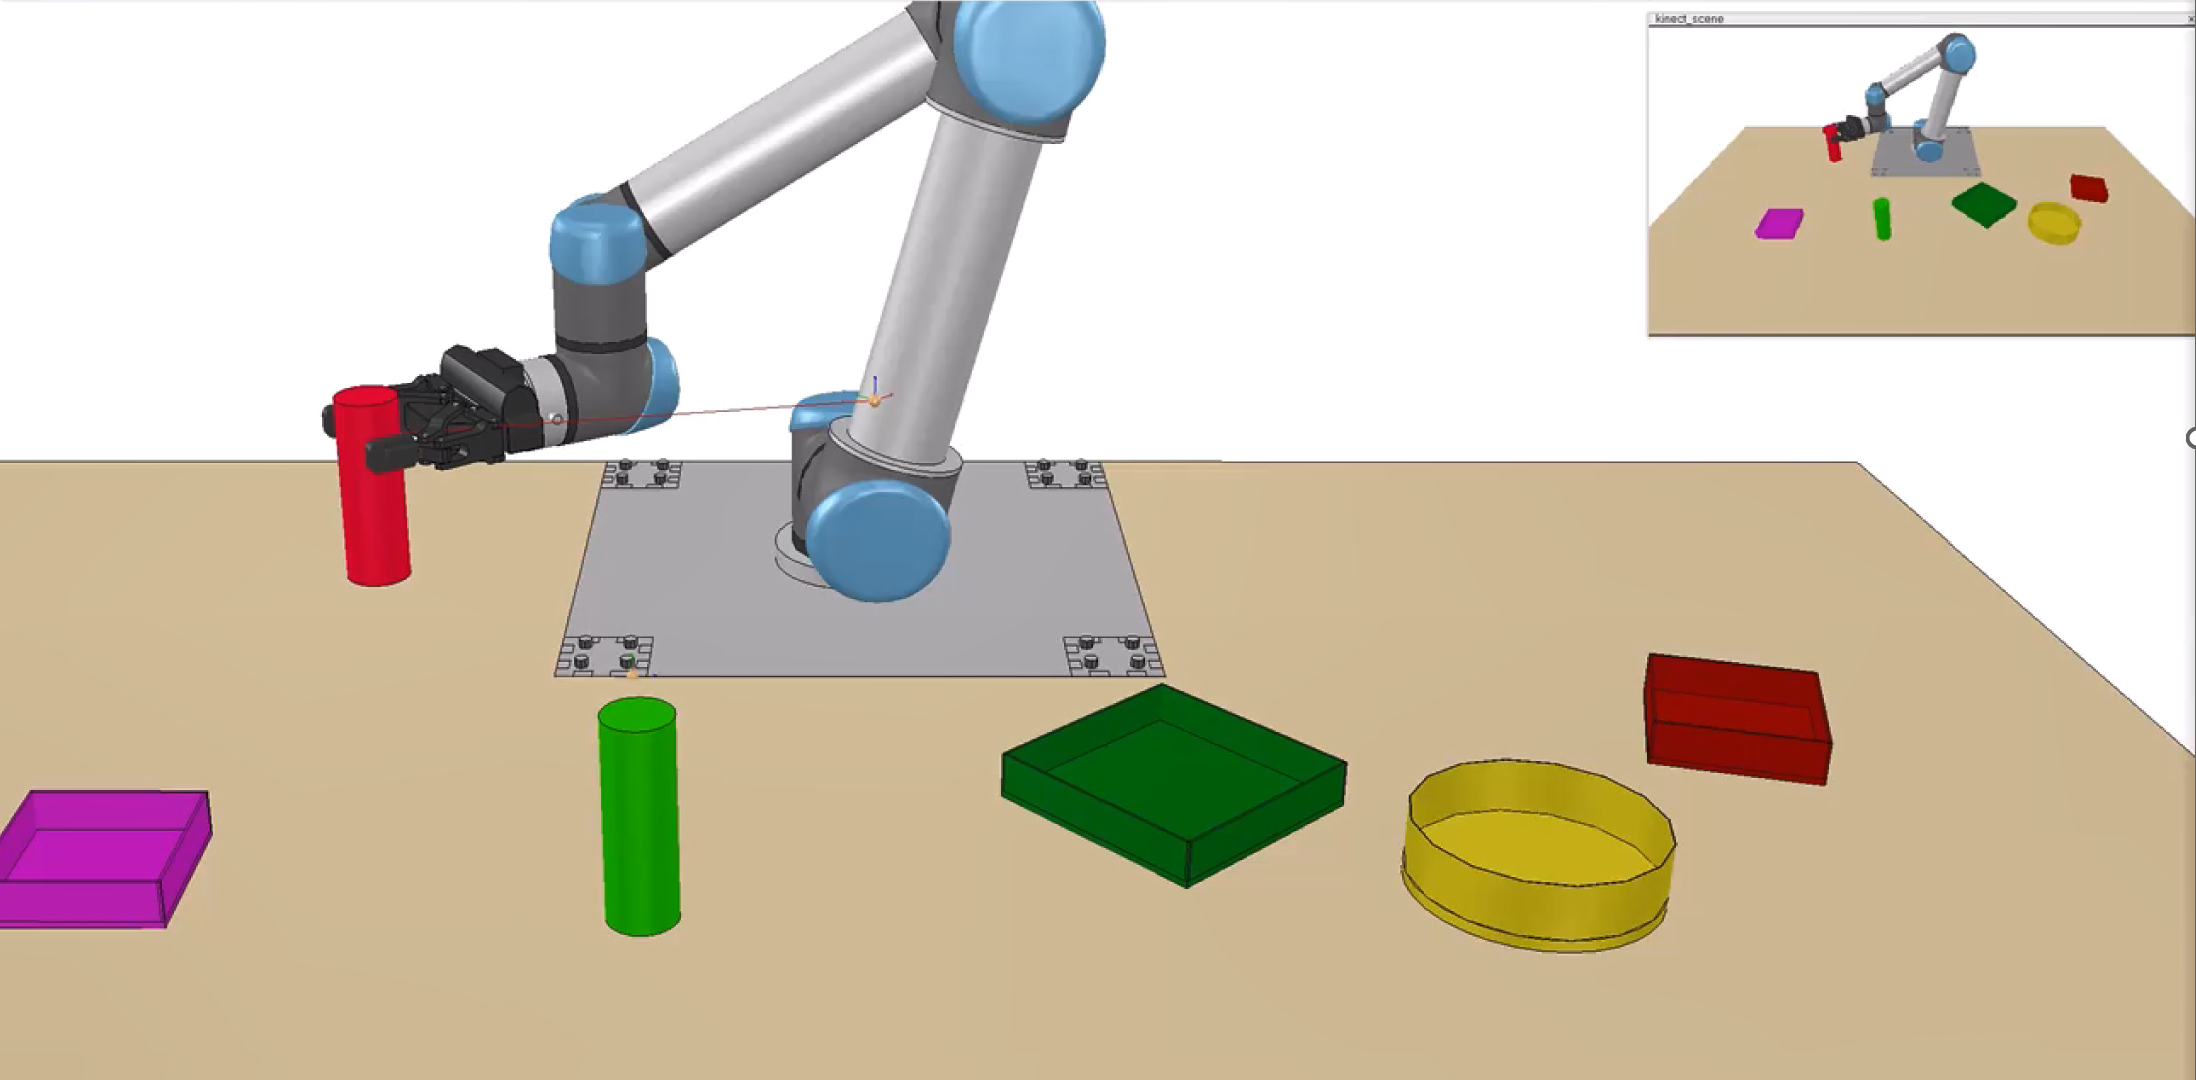
\includegraphics[width=\textwidth]{images/Language_Conditioned_Exp/theirs_1.png}
        \caption{Time step 60.}
    \end{subfigure}
    \begin{subfigure}[t]{0.18\textwidth}
        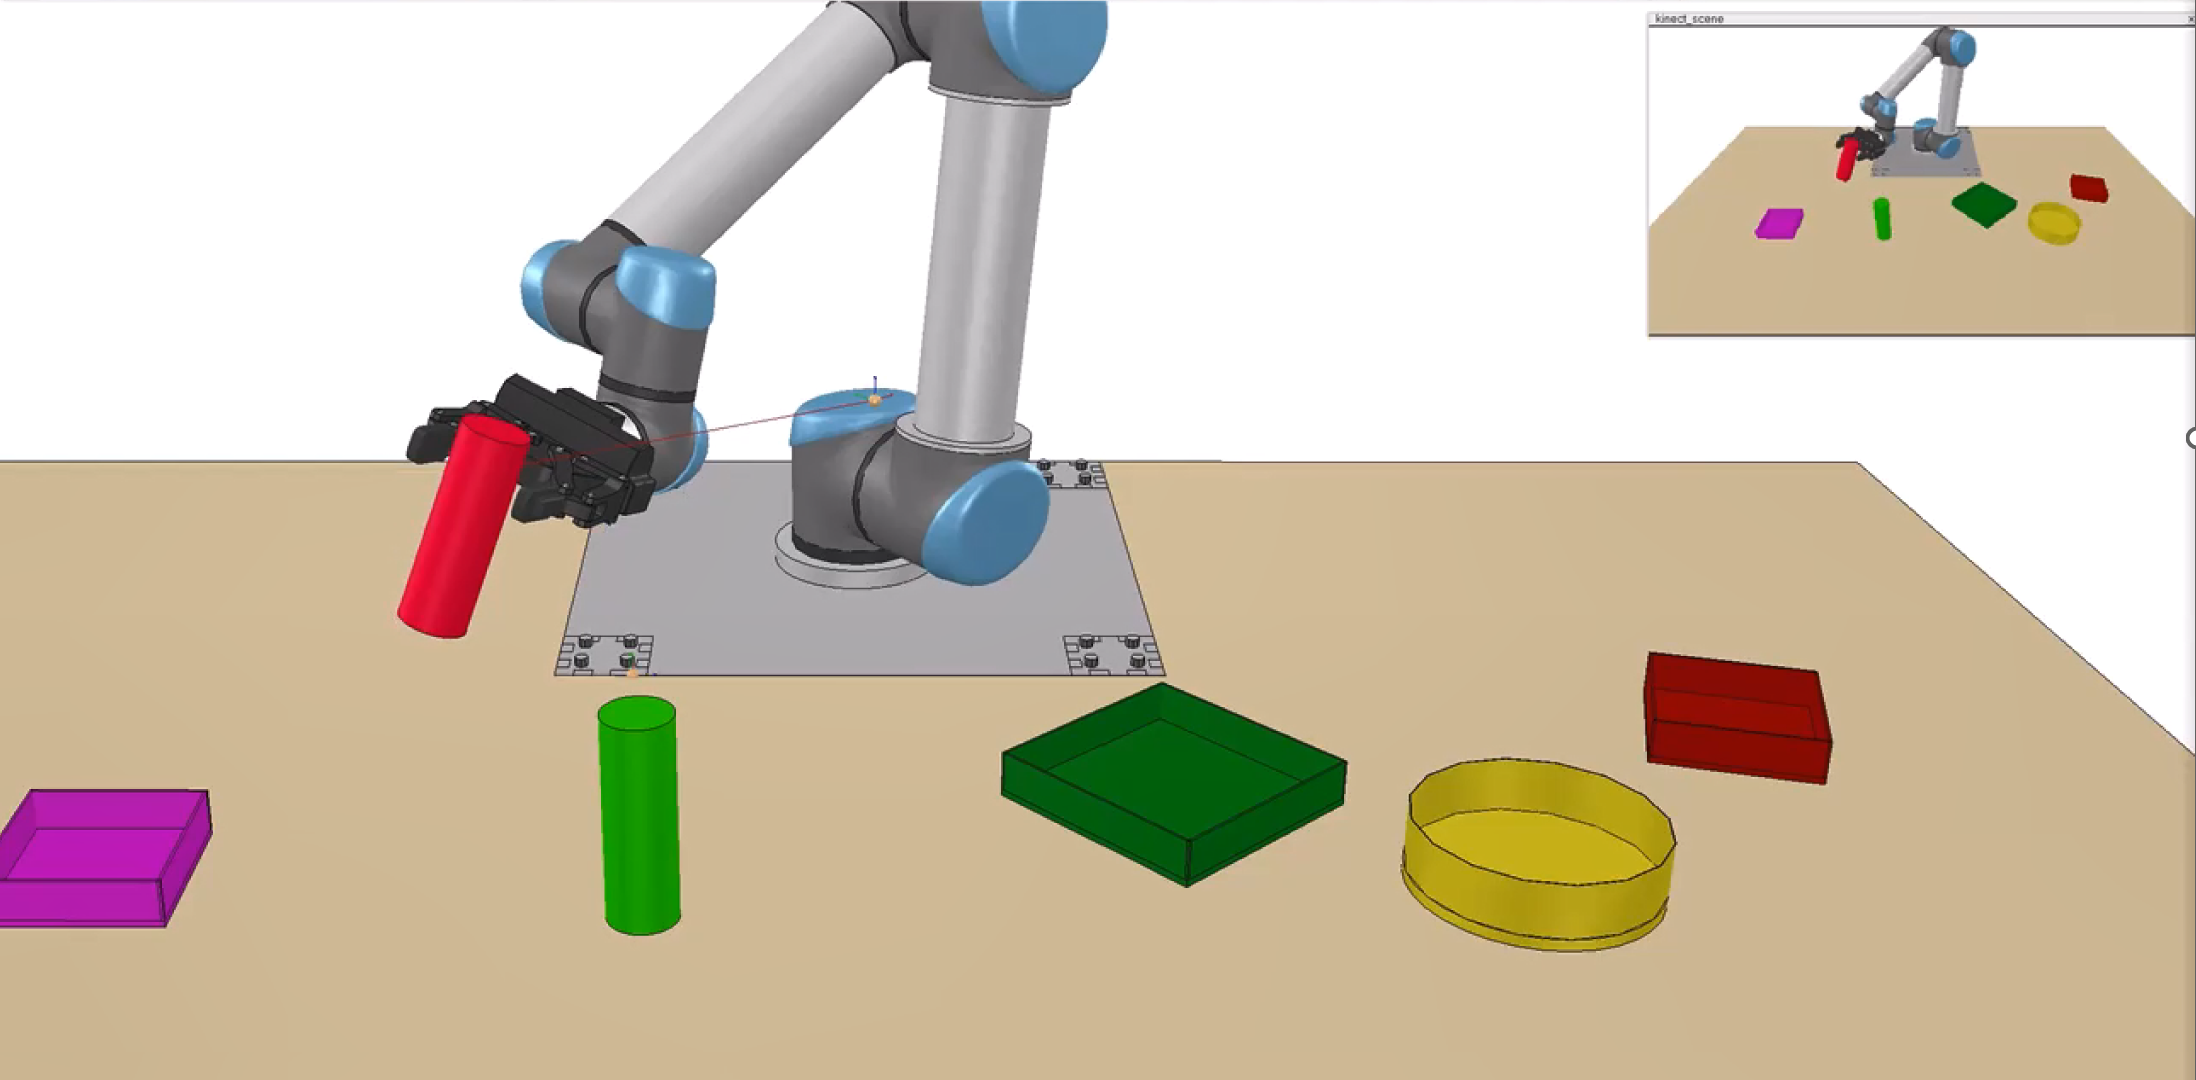
\includegraphics[width=\linewidth]{images/Language_Conditioned_Exp/theirs_2.png}
        \caption{Time step 120.}
    \end{subfigure}
    \begin{subfigure}[t]{0.18\textwidth}
        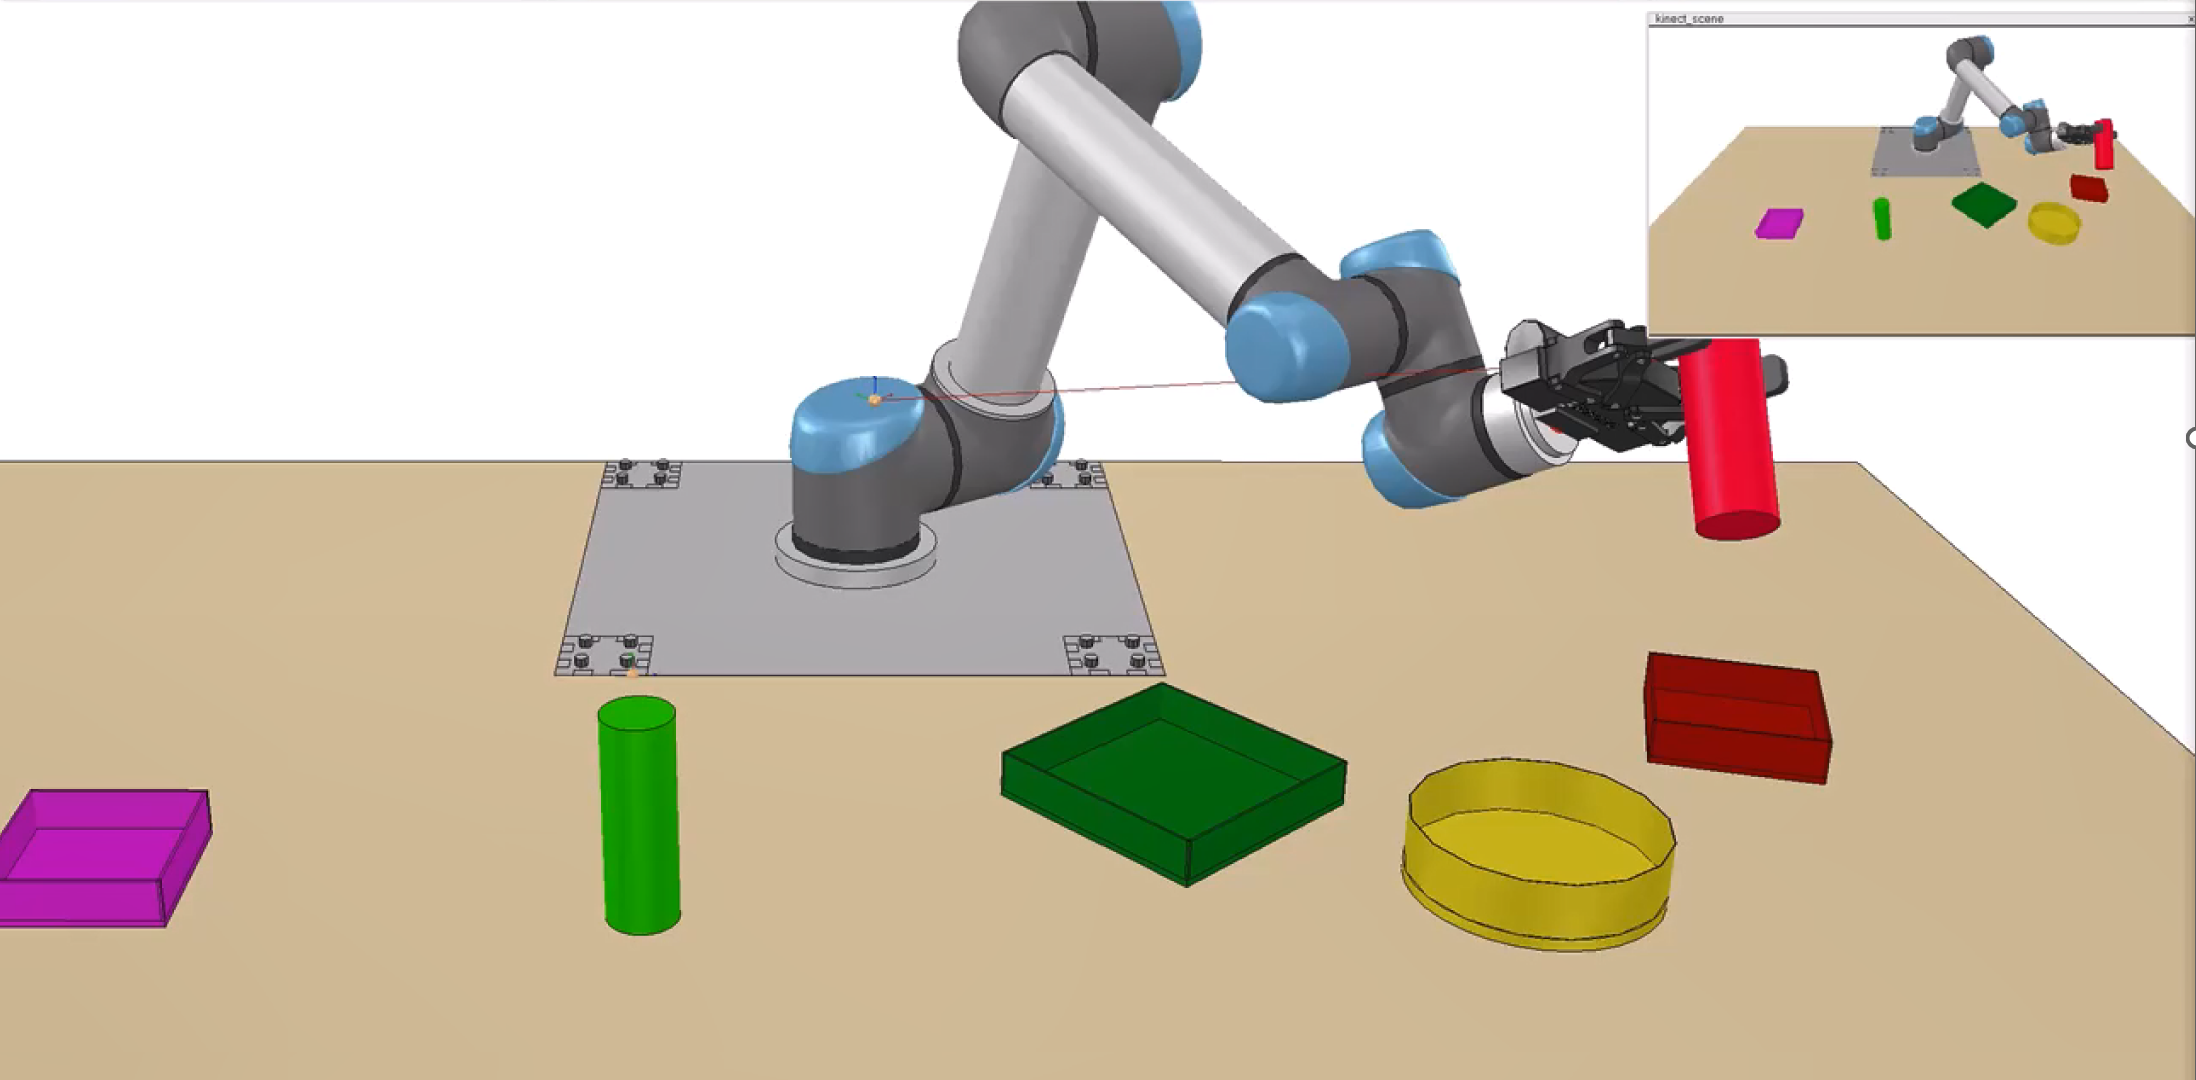
\includegraphics[width=\linewidth]{images/Language_Conditioned_Exp/theirs_3.png}
        \caption{Time step 180.}
    \end{subfigure}
    \begin{subfigure}[t]{0.18\textwidth}
        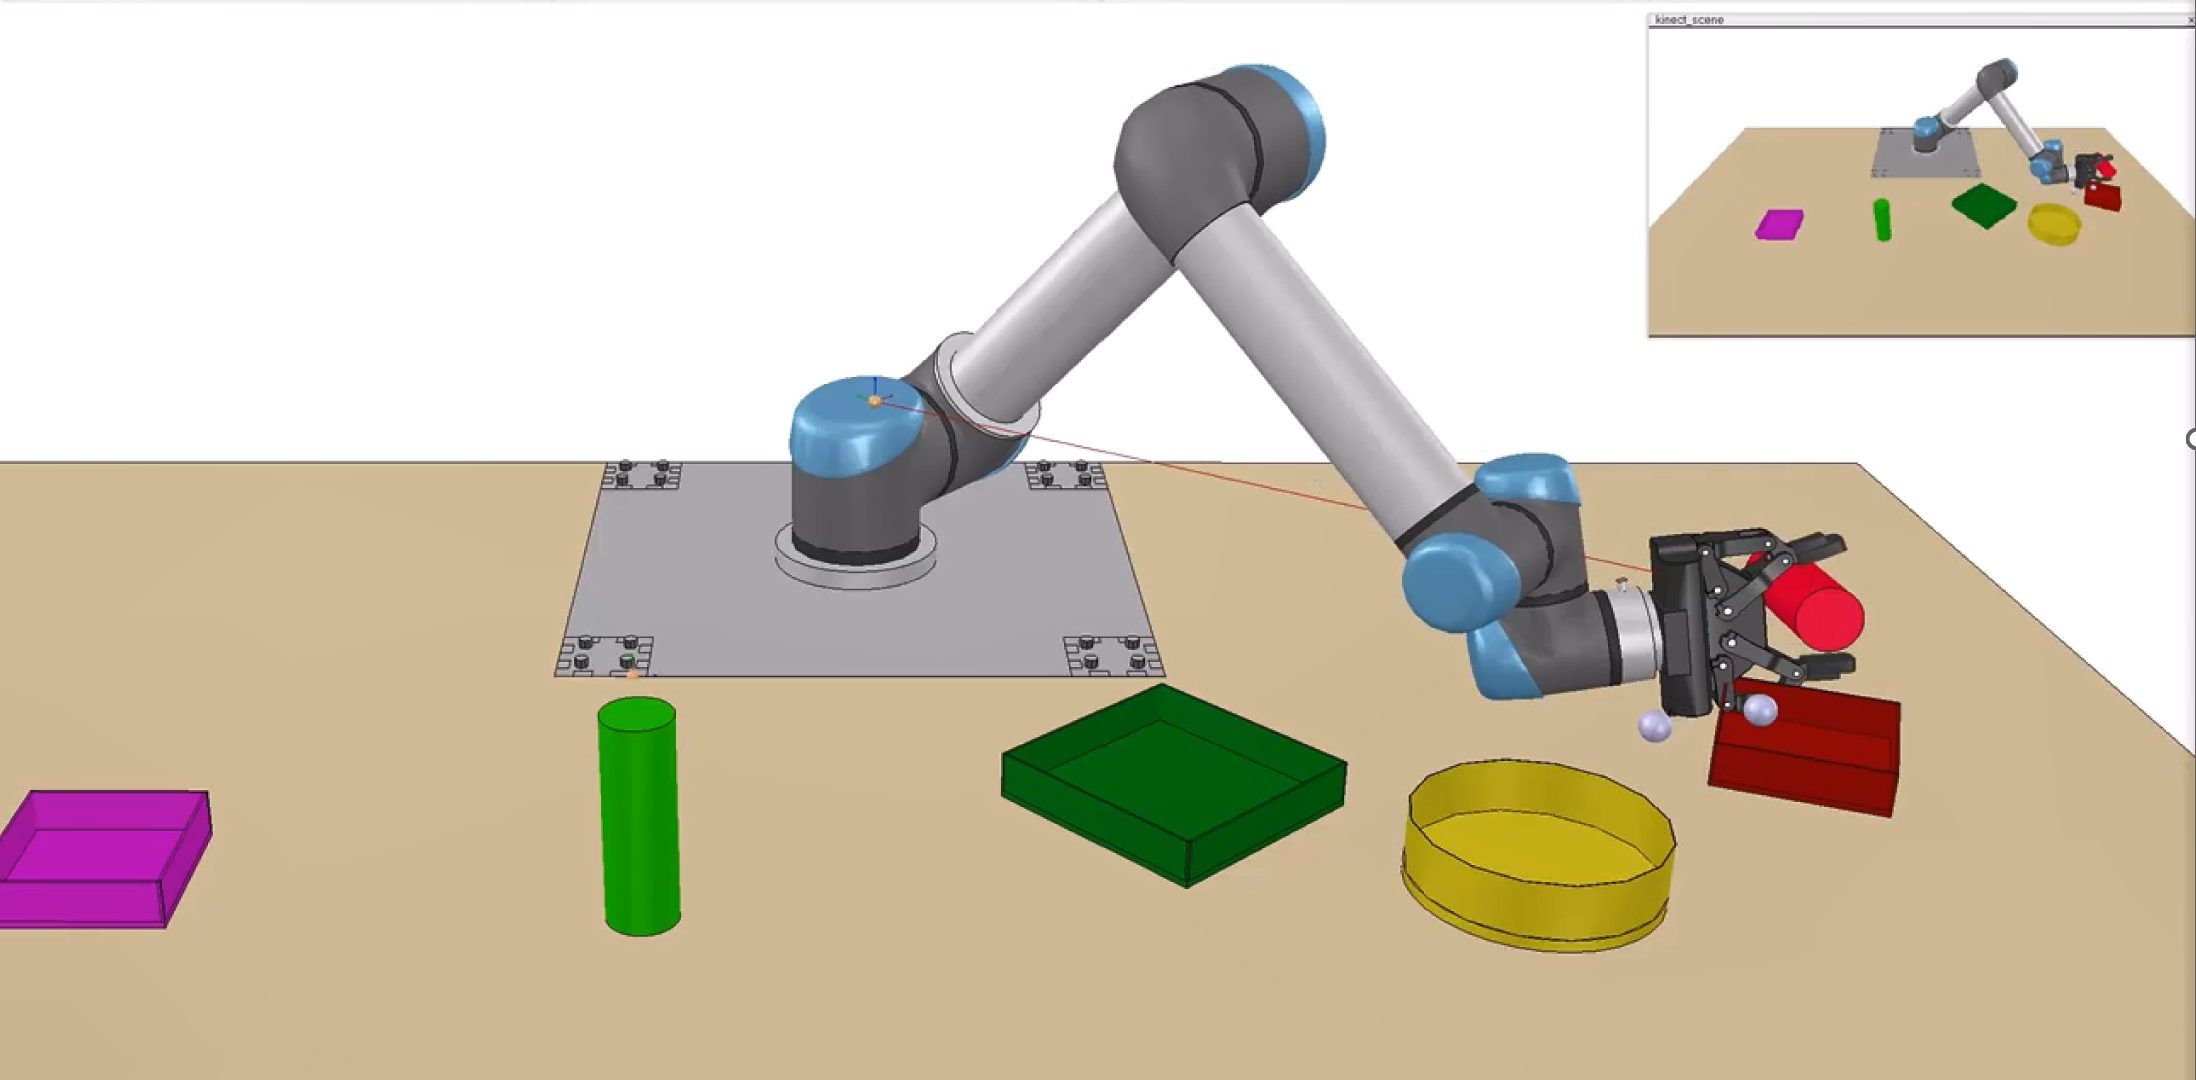
\includegraphics[width=\linewidth]{images/Language_Conditioned_Exp/theirs_4.png}
        \caption{Time step 240.}
    \end{subfigure}
    \begin{subfigure}[t]{0.18\textwidth}
        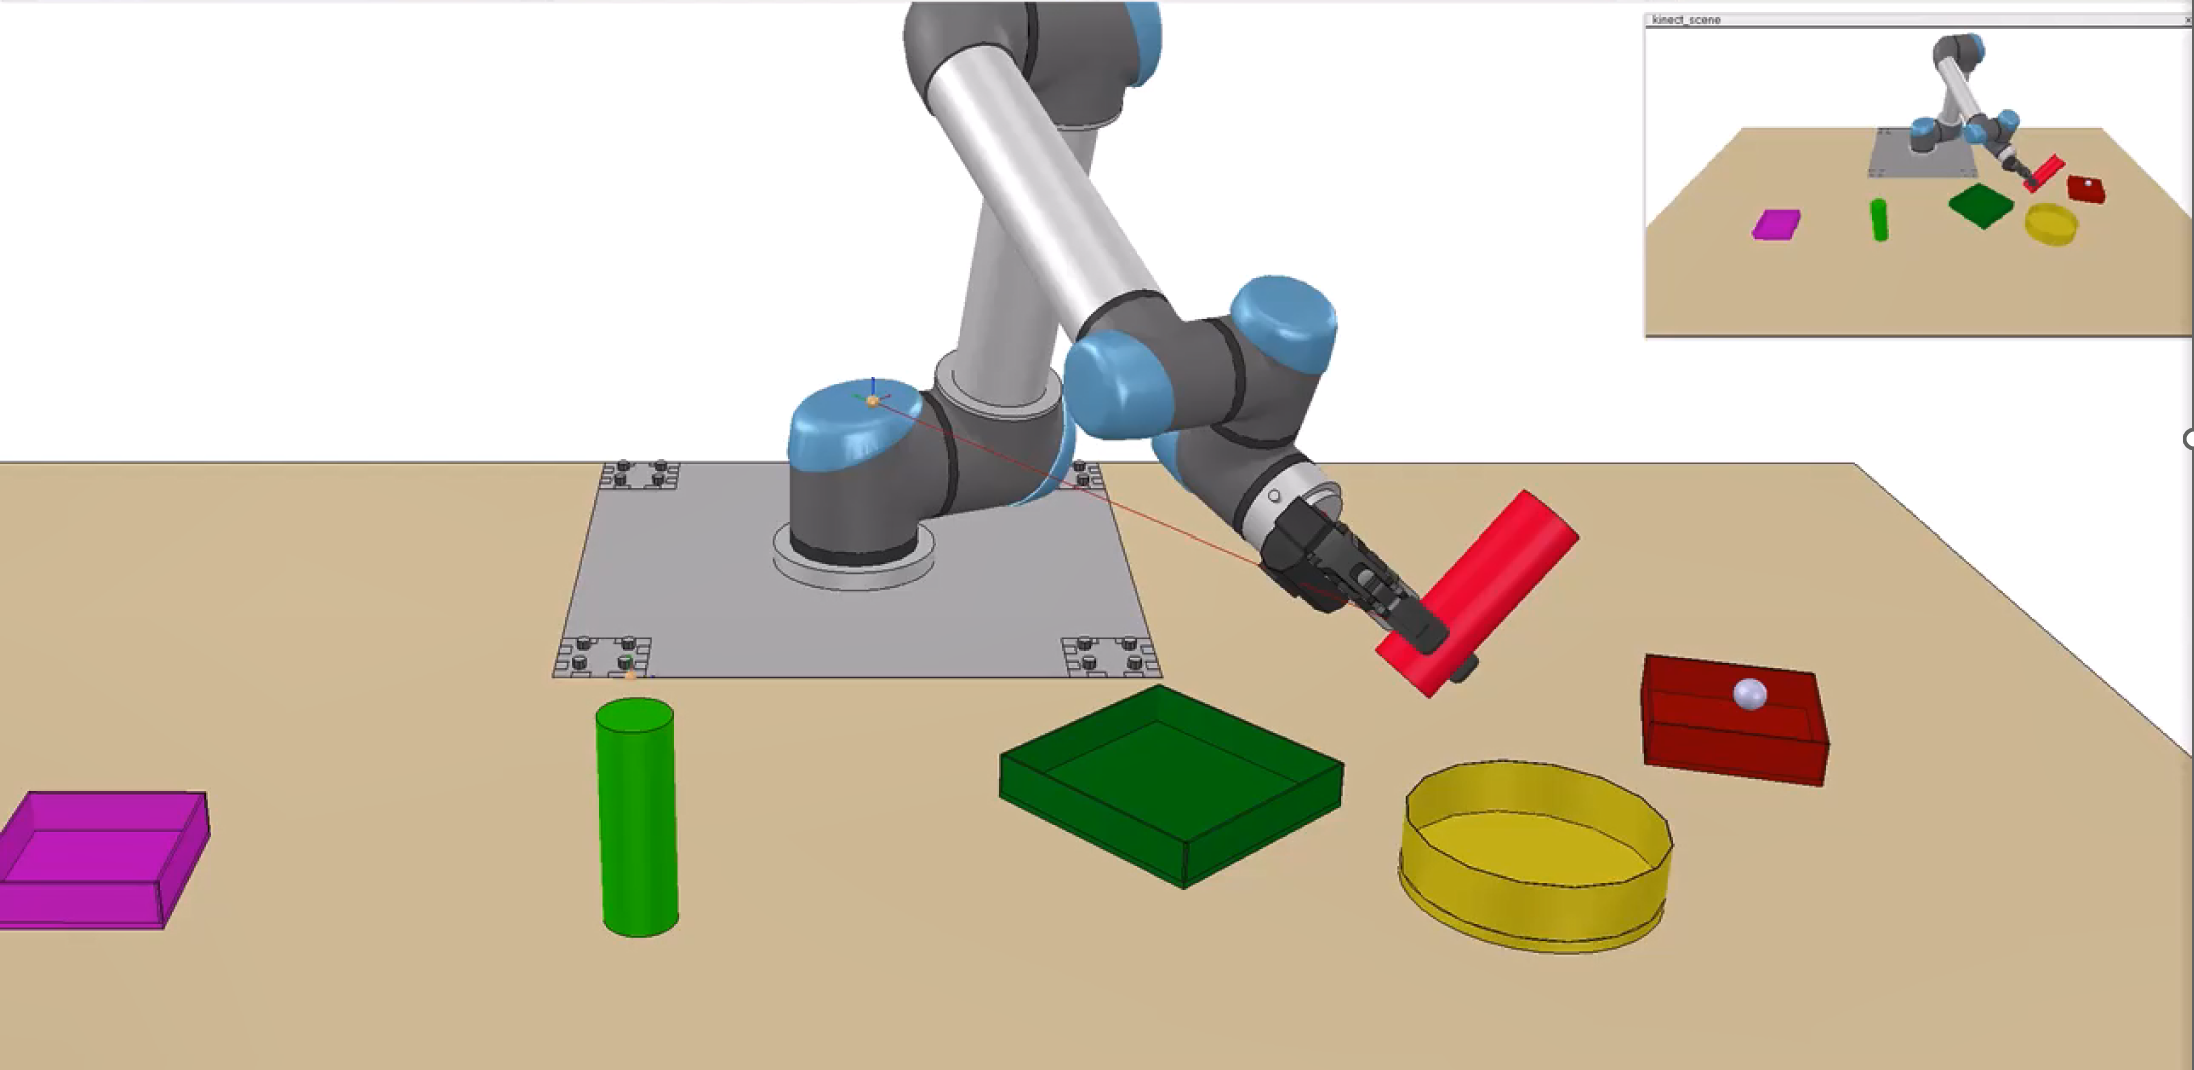
\includegraphics[width=\linewidth]{images/Language_Conditioned_Exp/theirs_5.png}
        \caption{Time step 300.}
    \end{subfigure}

    \bigskip % more vertical separation
    \begin{subfigure}[t]{0.18\textwidth}
        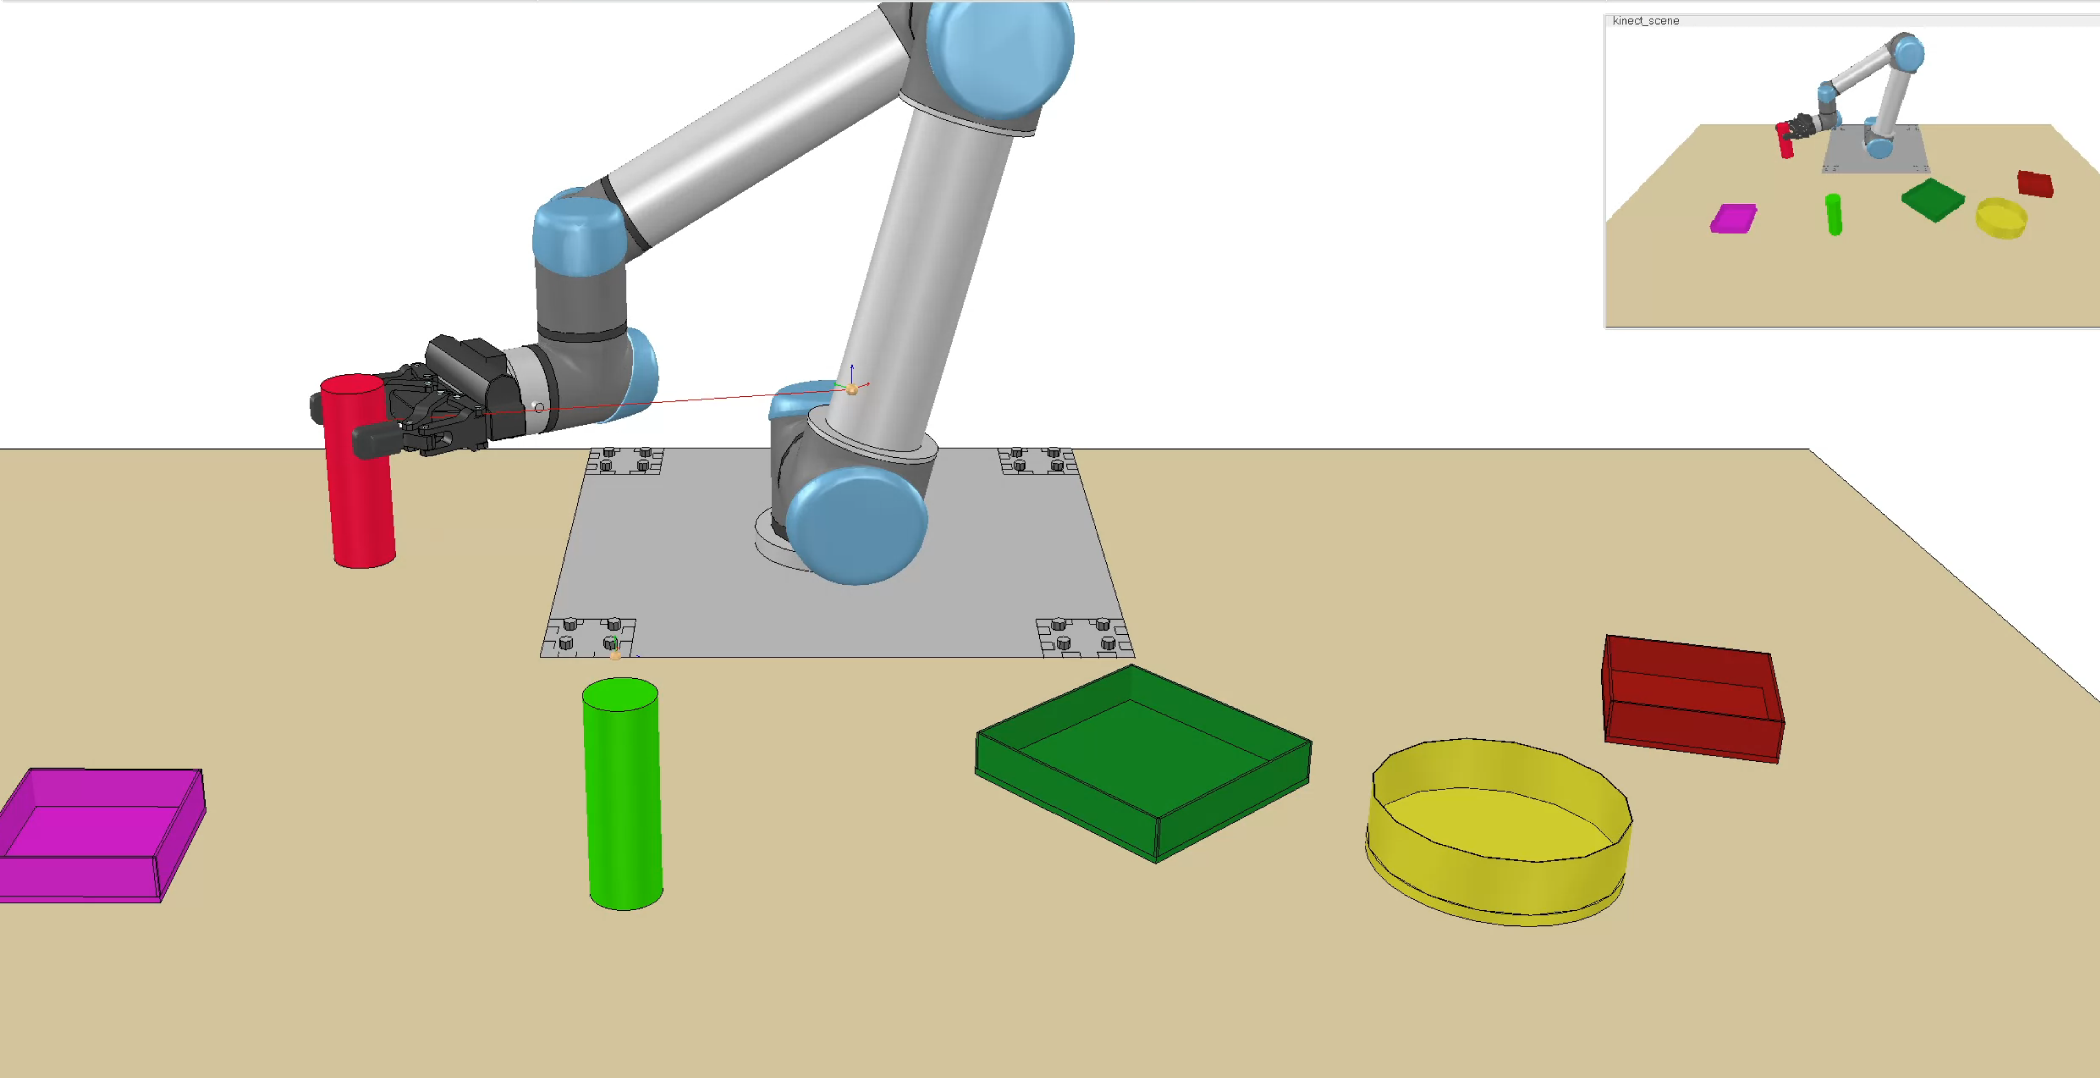
\includegraphics[width=\linewidth]{images/Language_Conditioned_Exp/mine_1.png}
        \caption{Time step 60.}
    \end{subfigure}
    \begin{subfigure}[t]{0.18\textwidth}
        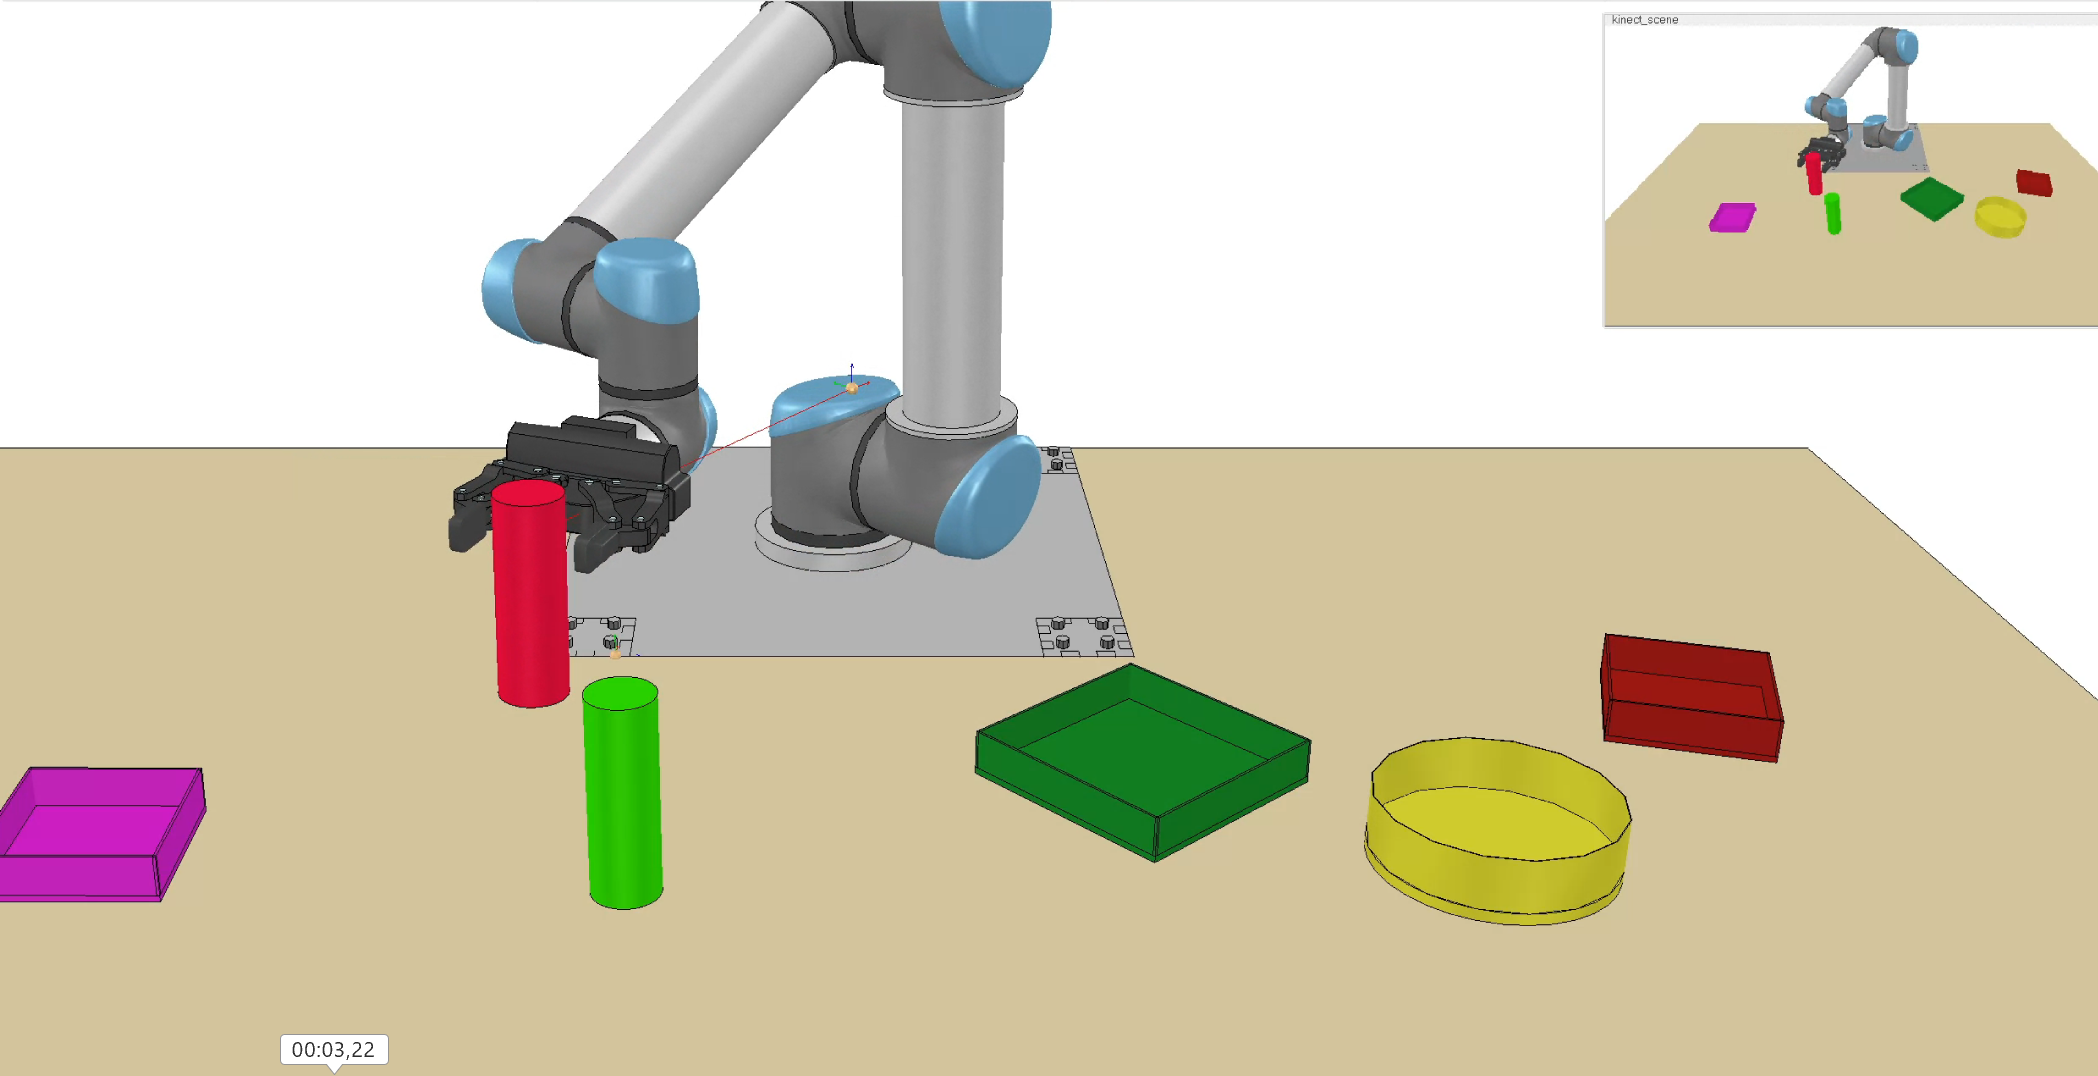
\includegraphics[width=\linewidth]{images/Language_Conditioned_Exp/mine_2.png}
        \caption{Time step 120.}
    \end{subfigure}
    \begin{subfigure}[t]{0.18\textwidth}
        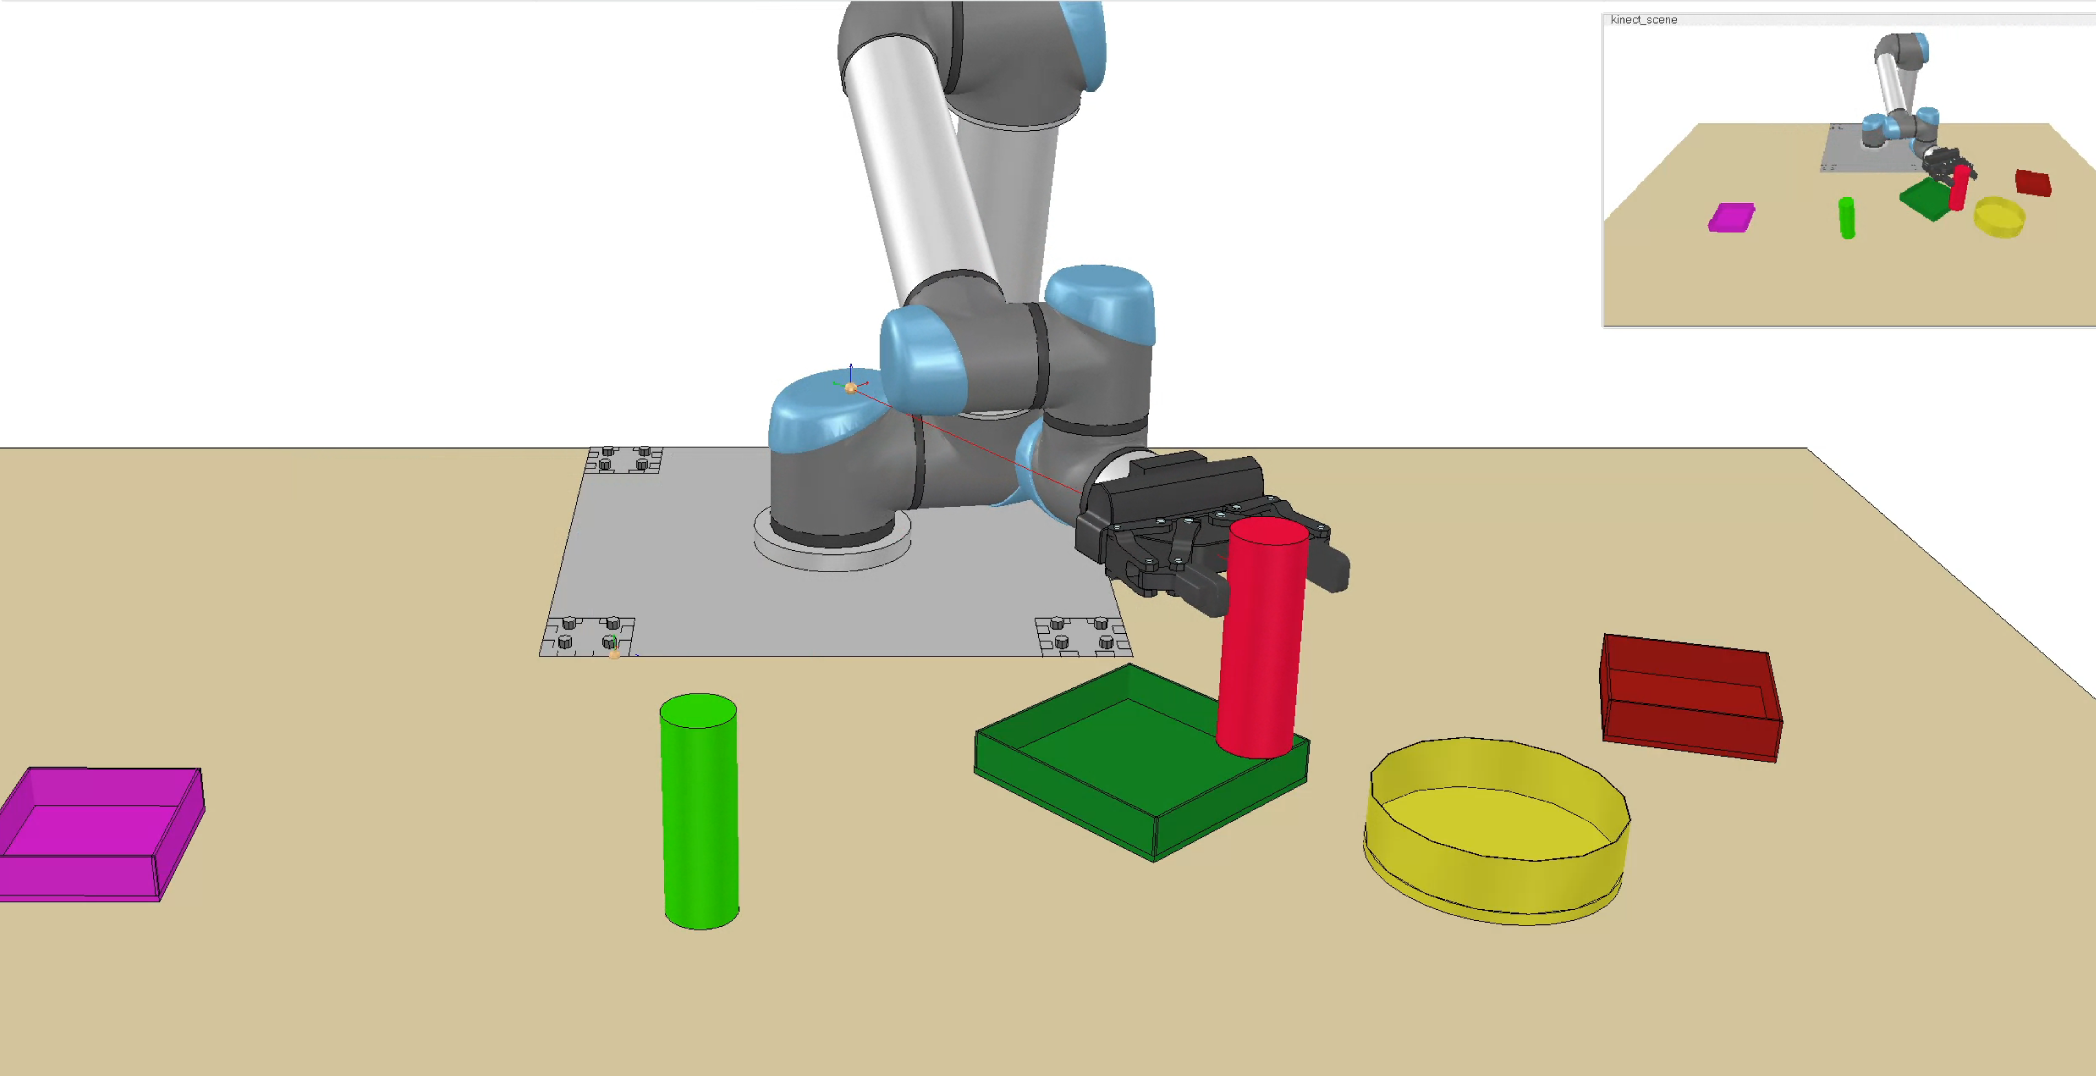
\includegraphics[width=\linewidth]{images/Language_Conditioned_Exp/mine_3.png}
        \caption{Time step 180.}
    \end{subfigure}
    \begin{subfigure}[t]{0.18\textwidth}
        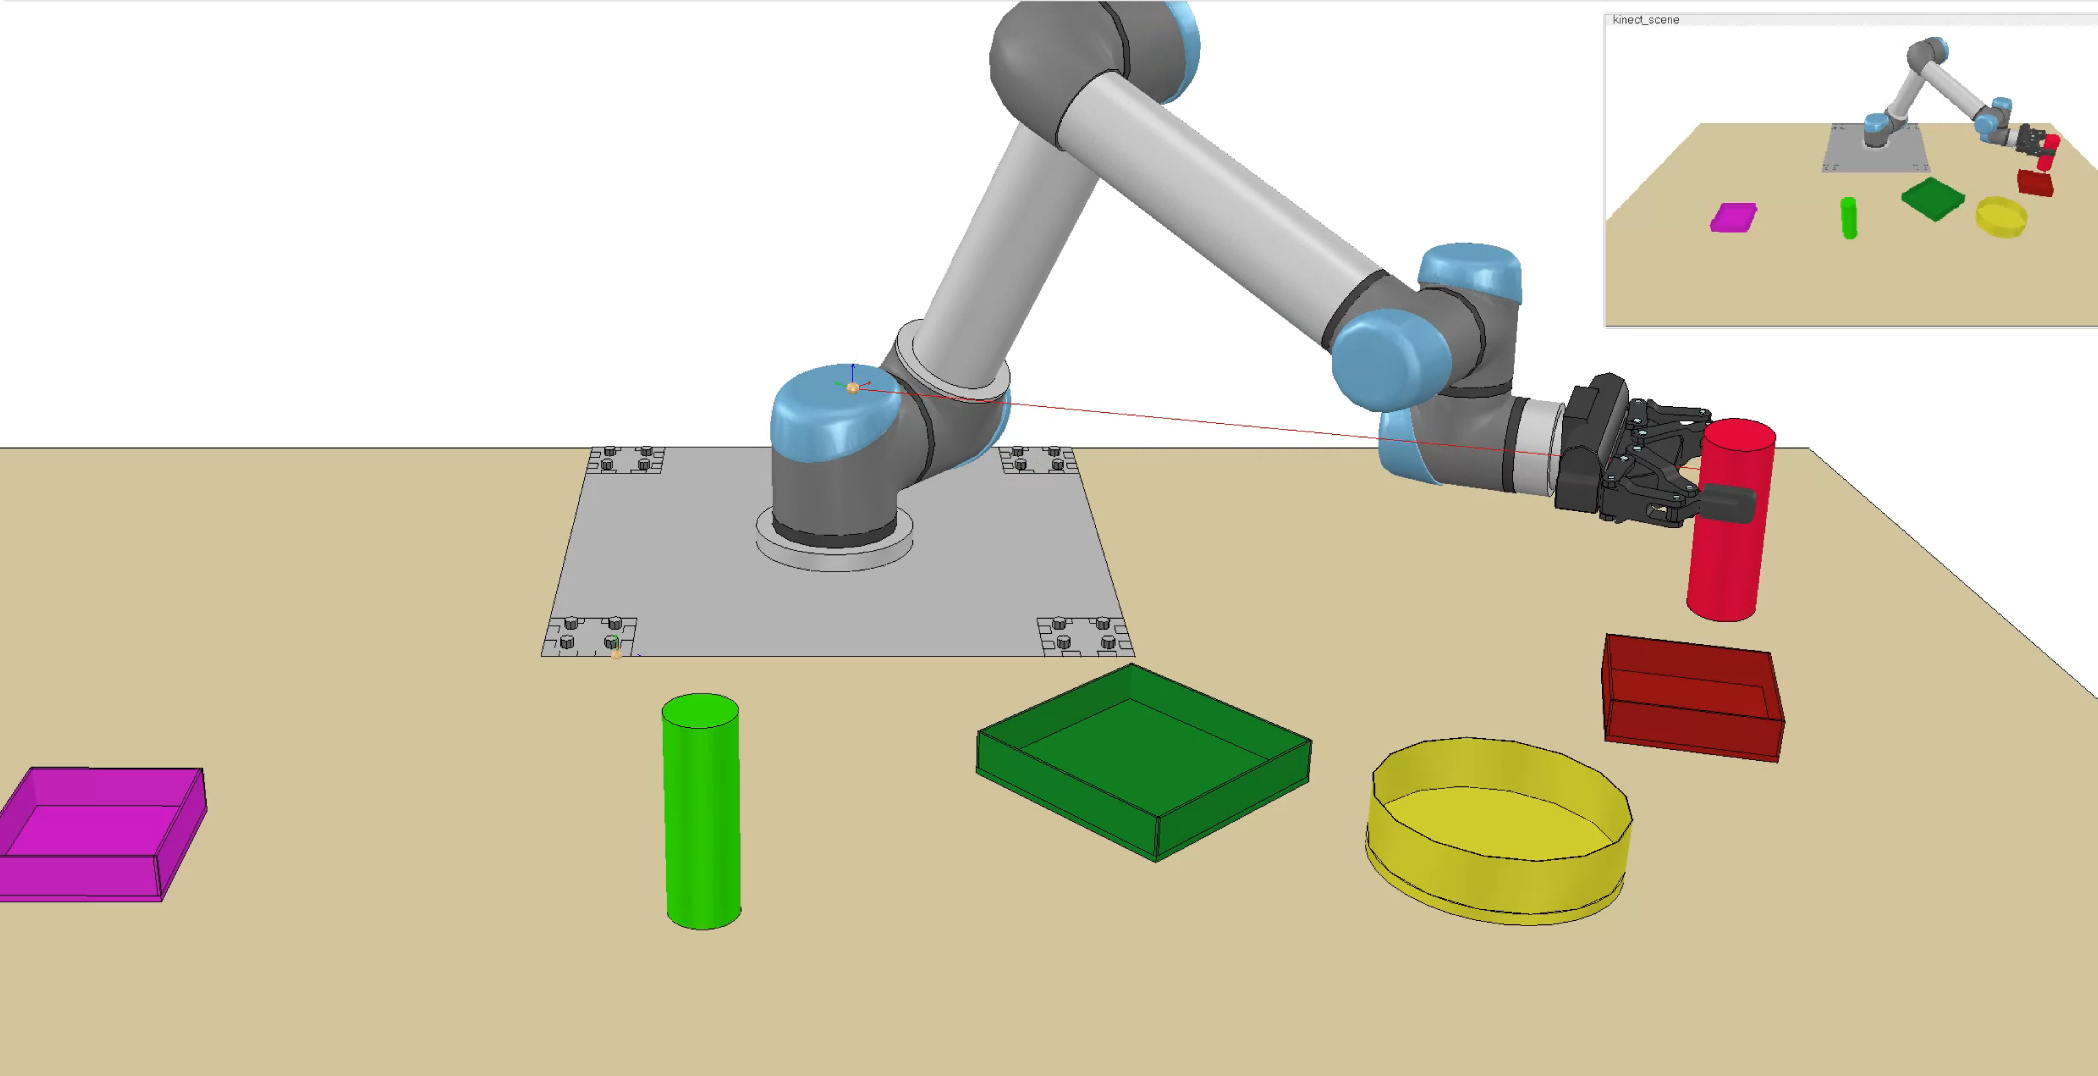
\includegraphics[width=\linewidth]{images/Language_Conditioned_Exp/mine_4.png}
        \caption{Time step 240.}
    \end{subfigure}
    \begin{subfigure}[t]{0.18\textwidth}
        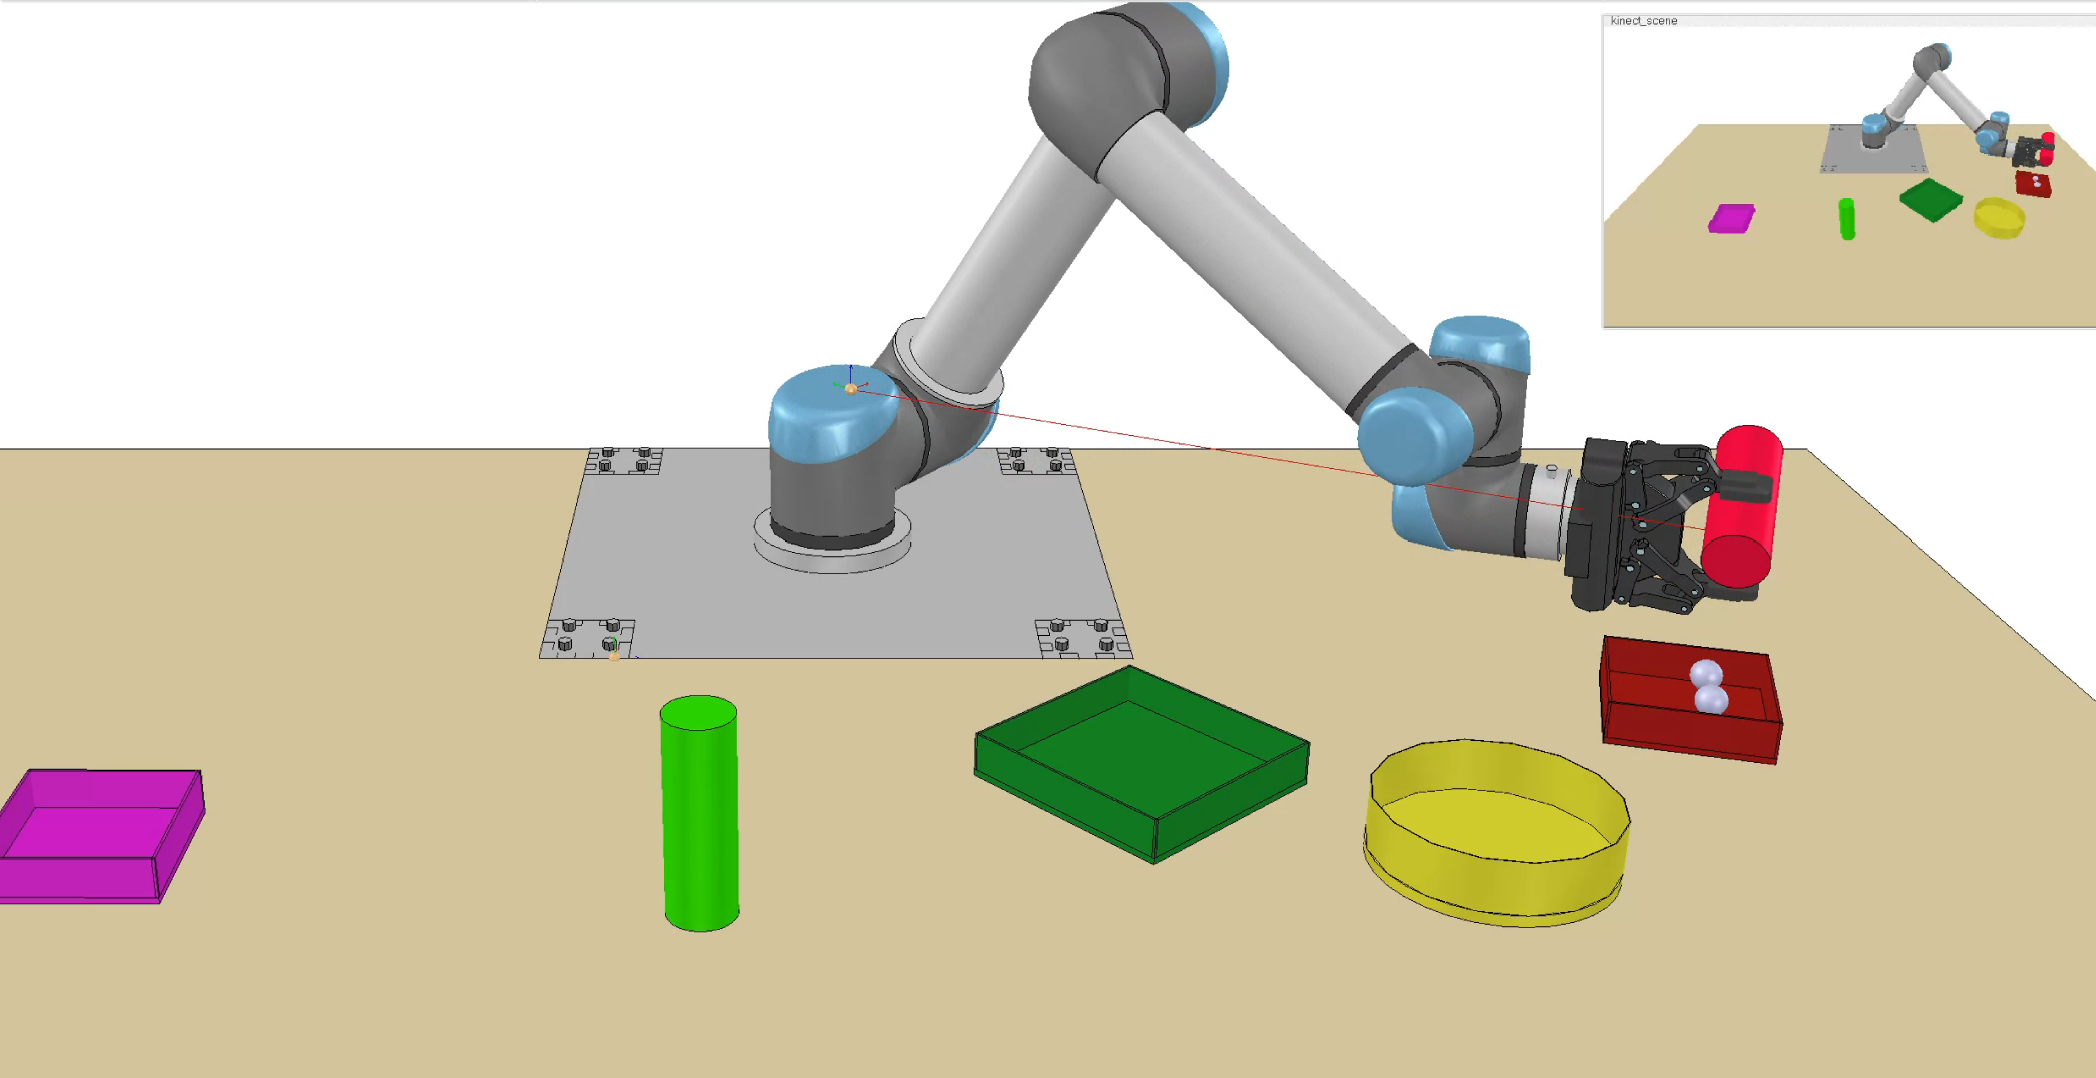
\includegraphics[width=\linewidth]{images/Language_Conditioned_Exp/mine_5.png}
        \caption{Time step 300.}
    \end{subfigure}
    \caption{Comparison of a pour task. The policy learned by the LCIL algorithm (top row) spills the content over the table and moves unpredictable. The task is considered a failure 
    by the benchmark, as most drops did not land in the goal bowl. Active Critic (bottom row) performs the task as intendet with no unexpected movement.}
    \label{fig: AC vs. Rec}
\end{figure}
Moreover in figure \ref{fig: AC vs. Rec} we have depicted a case in the test dataset, which our policy solved and compared it to the performce of the recurrent algorithm, which failed at the task. 
While our approach hit the target precisely, the recurrent model was widely off. We assume this is caused by the fact that during inference time, the 
i.i.d. assumption of the input data to the policy is broken. Intuitively, the recurrent policy 
is in a state that it has not seen before and acts slightly different to the expert movement. After some steps, the policy now sees inputs that are vastly 
different then the training distribution, thus it starts to act unpredictable. As argued in section \ref{COD_AC} this is an advantage of our policy, as it 
does not break the i.i.d. assumption.

\section{Meta World}
The Meta World benchmark is a challenging robot simulation benchmark...

We want to test two aspects of our algorithm
-fine tuning
-reinforcement learning

RPPO TQC PPO fine tuning, positional encoding, reasons why they were chosen.
We tested our algorithm on four environments from the Meta-World benchmark with variying complexity. 
PPO, TQC and RPPO were pretrained unsing behavioural cloning. We chose the best performing policy during behavioural cloning by testing the policy on 50 test 
trajectories every 400 full cycles through the 
expert transitions. Technically, these test trajectories were environment interactions, but we chose not to count them to give the best case comparison to the AC algorithm, which was not pretrained. 


\subsection{Fine Tuning}
In this section we analyze our algorithm in a fine tuning setup. We provided the algorithms with 4 and 15 expert demonstrations per environment and used a relatively short reinforcement learning phase 
with 400 sampled trajectory consisting of 100 steps each. One problem we wanted to overcome is "catastrophic 
forgetting" that can occure, when the data distribution shifts. During the imitation phase, the learners only sees positive examples sampled according to the distribution induced by the expert. 
In the reinforcement learning phase, the learner samples trajectories according to the actor of the learner, thus the distribution shift. Our algorithm is more robust to this problem, as it 
decouples the generator distribution, namely the distribution induced by the actor, from the training process, as discussed in section \ref{inference_time_planning}. We present our findings in 
figure \ref{fig:finetuning}. For the environments "Pick and Place" and "Push" we show the plots 
for 15 expert demonstrations, as we found 4 expert demonstrations were not enough to meaningfully learn within 400 training episodes. The environments "Reach" and "Window Open" are easier to learn, 
so we display the experiments with 4 expert demonstrations each, as giving 15 expert demonstrations lead to near pefect performance from imitation learning alone. All plots for all experiments can 
be found in Appendix \ref{chapter:additional_plots}. 
We find, that AC is the only algorithm that can meaningfully improve it's perforance given the limited amount of environment interactions. RPPO is a recurrent algorithm and is the most sensitive to hyper parameter tuning. 
We expected RPPO to be the least performant from our discussion of the curse of dimensionality in section \ref{COD_AC}. The algorithms guided by GAIL did not improve meaningfully. We assume the limited 
amount of environment interaction was not proficcient to learn a good discriminator and improve the policies. We tried differnt hyper parameter settings, including fine tuned parameters for the 
environments but for dense rewards and observations from the [hyper parameter ZOO]. We found that the performance was most relient on the learning rate. Too high values lead to catastrophic forgetting. Some cases can be seen in 
the appendix \ref{chapter:additional_plots}, where we were not able to find suitable hyper parameters. The values we chose were the highest values before pratically no learning took place, however 
mostly the performance decreased, anyway.


\begin{figure}[htbp]
    \centering
    \begin{subfigure}[t]{0.45\textwidth}
      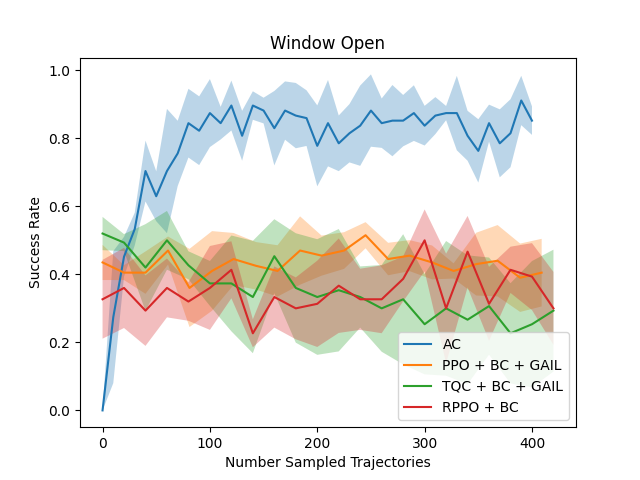
\includegraphics[width=\textwidth]{images/FineTuning/Window Open.png}
      \caption{Window Open environment, 4 expert demonstrations.}
      \label{fig:plot3}
    \end{subfigure}
    \begin{subfigure}[t]{0.45\textwidth}
      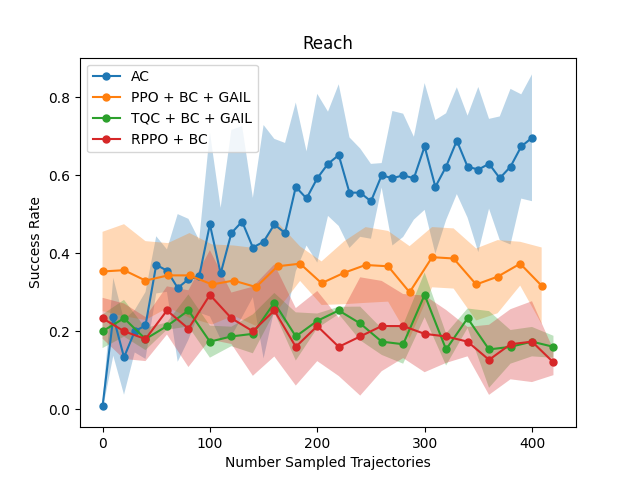
\includegraphics[width=\textwidth]{images/FineTuning/Reach.png}
      \caption{Reach environment, 4 expert demonstrations.}
      \label{fig:plot1}
    \end{subfigure}
    \medskip
    \begin{subfigure}[t]{0.45\textwidth}
      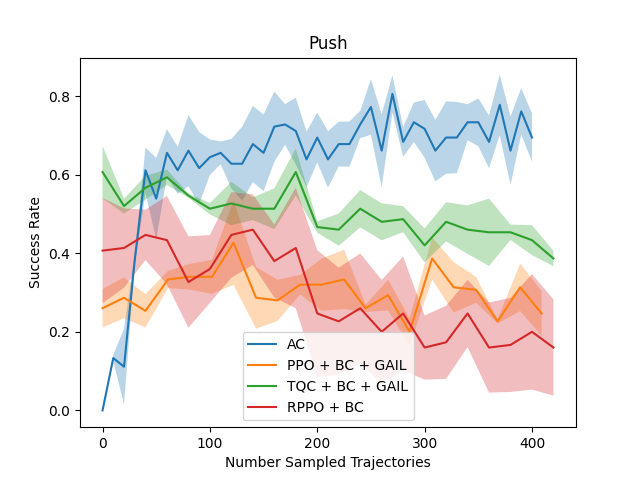
\includegraphics[width=\textwidth]{images/FineTuning/Push.png}
      \caption{Push environment, 15 expert demonstrations.}
      \label{fig:plot2}
    \end{subfigure}
    \begin{subfigure}[t]{0.45\textwidth}
      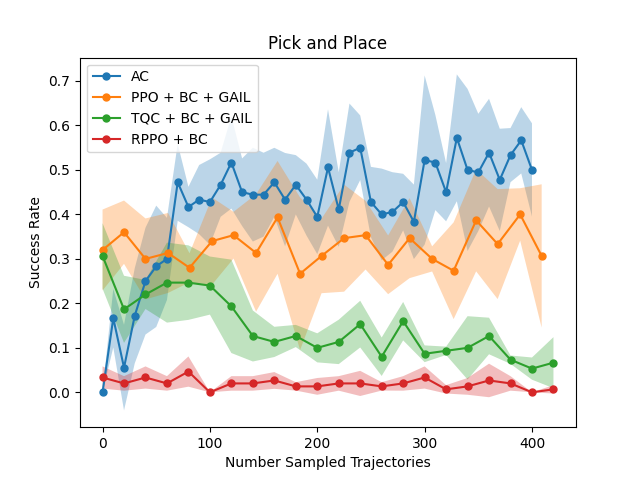
\includegraphics[width=\textwidth]{images/FineTuning/Pick and Place.png}
      \caption{Pick and Place environment, 15 expert demonstrations.}
      \label{fig:plot4}
    \end{subfigure}
    \caption{
    The learner trained by GAIL and RPPO were pretrained using behavioural cloning with the given number of expert demonstrations. 
    The x-axis shows the number of sampled environment epsiodes, each with 100 steps.  One initial observation and a sparse reward signal at the end of each episode was provided.}
    \label{fig:finetuning}
\end{figure}

\subsection{Guided Reinforcement Learning}
In this section, we test the perforance of AC given only one expert trajectory. We use the Reach and Winow Open environments with 2000 training epsiodes per run and two runs per experiment and learner. 
Per data point we sampled 50 trajectories from the test data set. 
In this setting, the algorithms must learn most of the behaviour from reinforcement learning, but the initial expert 
demonstration is useful to overcome the initial search problem. We only provide sparse reward and one obervsation per trajectory, thus finding the first viable solution by unguided 
trial and error is unviable for most problems. For the baselines, we used RPPO, PPO and TQC with behavioural cloning as pretraining. We expect TQC to be better at exploration and PPO to be more stable. The results 
are shown in figure \ref{fig:guided_ref}. 

\begin{figure}[htbp]
    \centering
    \begin{subfigure}[b]{0.45\textwidth}
      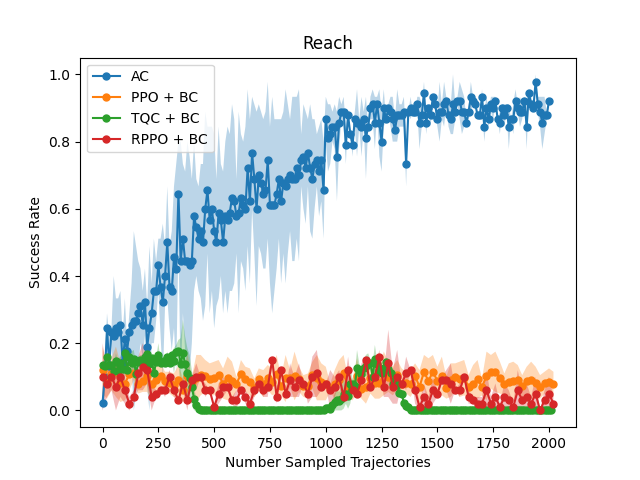
\includegraphics[width=\textwidth]{images/1_2000/Reach.png}
      \caption{Reach environment. Comparison of the different learners.}
    \end{subfigure}
    \hfill
    \begin{subfigure}[b]{0.45\textwidth}
      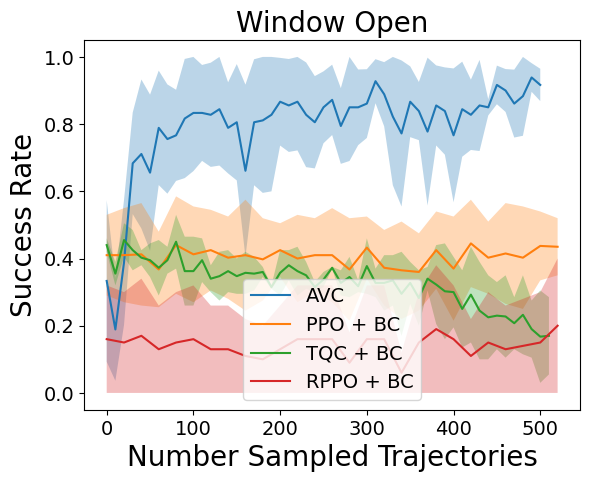
\includegraphics[width=\textwidth]{images/1_2000/Window Open.png}
      \caption{Window Open environment. Comparison of the different learners.}
    \end{subfigure}
    \medskip
    \begin{subfigure}[b]{0.45\textwidth}
      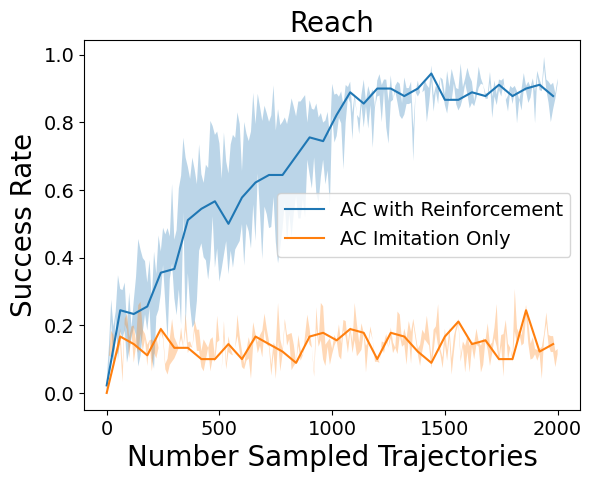
\includegraphics[width=\textwidth]{images/1_2000_imi/Reach.png}
      \caption{Reach environment. Comparison between pure imitation learning and reinforcement learning.}
    \end{subfigure}
    \hfill
    \begin{subfigure}[b]{0.45\textwidth}
      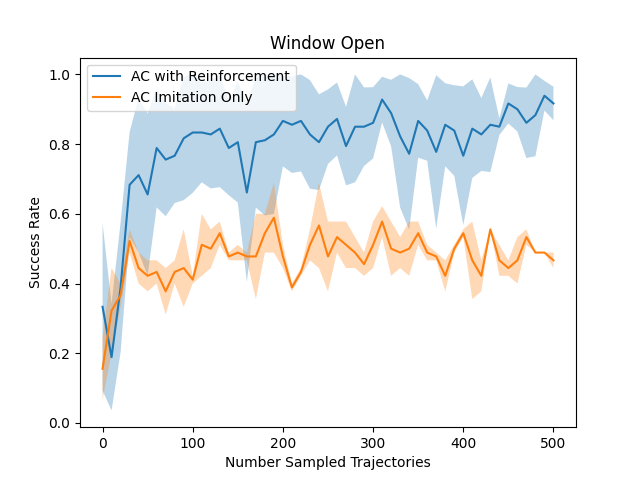
\includegraphics[width=\textwidth]{images/1_2000_imi/Window Open.png}
      \caption{Window Open environment. Comparison between pure imitation learning and reinforcement learning.}
    \end{subfigure}
    \caption{Each learner had access to one expert demonstration. 
    The learner trained by PPO, RPPO and TQC were pretrained using behavioural cloning given one demonstration. 
    The x-axis shows the number of sampled environment epsiodes, each with 100 steps. One initial observation and a sparse reward signal at the end of each episode was provided 
    during the reinforcement phase. The pure imitation learning experiments on the buttom row were conducted using no additional epsiodes from the environment. There, the x-axis 
    displays equal amount of compute compared to the reinforcement learning algorithm.
    The y-axis shows the success rate. Each experiment was repeatet twice with 
    50 sampled validation episodes per run and data point. The shaded region displays one standard deviation.}
    \label{fig:guided_ref}
\end{figure}

The AC algorithm was able to solve both environments with high success rates after 2000 sampled trajectories. TQC found a policy with about $20 \%$ success rate in the Reach environment after
about 1250 epsiodes in both runs, but did not outperform behavioural cloning. PPO was the most stable algorithm, as it did not drop below the initial performance from 
BC, but did not greatly improve. In the reach environment, no algorithm accept AC was able to improve above $20 \%$ perforance. In the windowopen environment, PPO and TQC achieved about $40 \%$ 
success rate. AC was able to achieve above $90 \%$ success rate in both environments. \\
Next we wanted to rule out, that the observed perforance gain of AC over the baselines comes mostly from the different underlying neural network architectures. AC uses transformers for the actor and 
critic, while the TQC and PPO implementations use MLPs and the RPPO implementation uses a GRU. To do this, we tested the performance of AC using pure imitation learning shown on the bottom row of 
figure \ref{fig:guided_ref}. We expect the main improvement of behavioural cloning in AC, TQC and PPO over a recurrent policy comes from the sequence encoding, as proposed in section \ref{COD_AC}.
We find that the pure imitation learning performance 
of AC is about the same as behavioural cloning for PPO and TQC. While in the Window Open environment, both PPO and TQC outperformed RPPO, we find that in the Reach environment RPPO performs 
similar to PPO. As only one expert trajectory was provided and we could only repeat the experiment twice out of time constraints, we find the difference between RPPO, PPO and TQC in the Reach 
environment too small to make conclusion about their relative perforance. \\
Overall, we take this finding as evidence for the effectiveness of the AC algorithm. It is highly unlikely that the observed improvement 
over the baselines comes mostly from the transformer architecture underlying the AC actor and critic, given the similar behavioural cloning perforance and the fact that our algorithms trains the actor and 
critic in a behavioural cloning style.  


\begin{figure}[htbp]
    \centering
    \begin{subfigure}[t]{0.65\textwidth}
      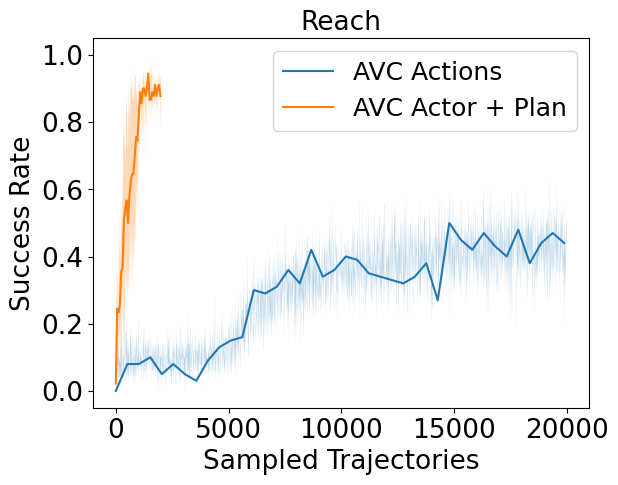
\includegraphics[width=\textwidth]{images/Plan_vs_Actions/Reach.png}
      \caption{Reach environment. Shown is the difference in learning efficiency of the Active Critic algorithm using two different optimisation modes.}
      \label{fig:plot1}
    \end{subfigure}
    \medskip
    \begin{subfigure}[t]{0.45\textwidth}
      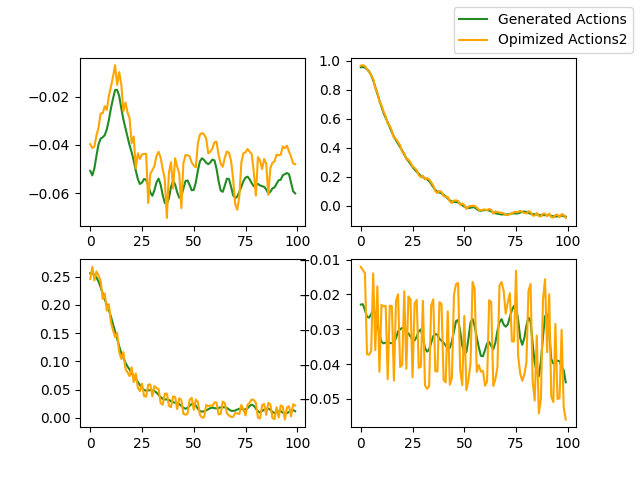
\includegraphics[width=\textwidth]{images/Plan_vs_Actions/changes/actions_1.png}
      \caption{Optimized trajectories (orange) and trajectories proposed by the actor (green). The gradient from the critic was applied to the actions.}
      \label{fig:plot2}
    \end{subfigure}
    \hfill
    \begin{subfigure}[t]{0.45\textwidth}
      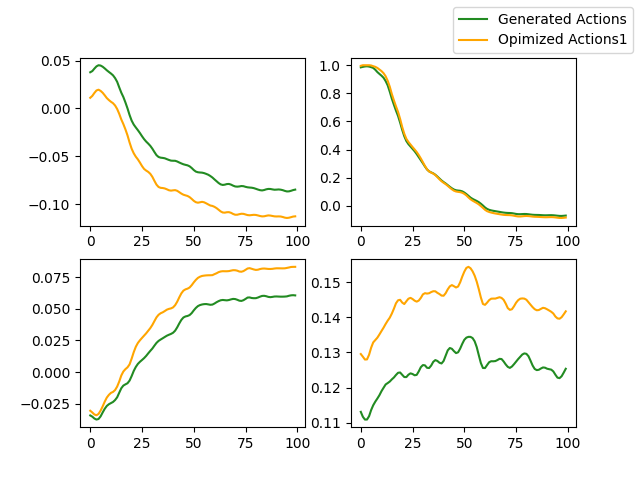
\includegraphics[width=\textwidth]{images/Plan_vs_Actions/changes/plans_actor_0.png}
      \caption{Optimized trajectories (orange) and trajectories proposed by the actor (green). The gradient from the critic was applied to the actor and planner.}
      \label{fig:plot4}
    \end{subfigure}
    \caption{Comparison of two different optimisation modi. Each experiment was repeated twice with 30 evaluation episodes per data point.
    The x-axis shows the number of sampled environment epsiodes, each with 100 steps. One initial observation and a sparse reward signal at the end of each episode was provided.}
    \label{fig:fourplots}
\end{figure}

\begin{figure}[htbp]
    \centering
    \begin{subfigure}[b]{0.45\textwidth}
      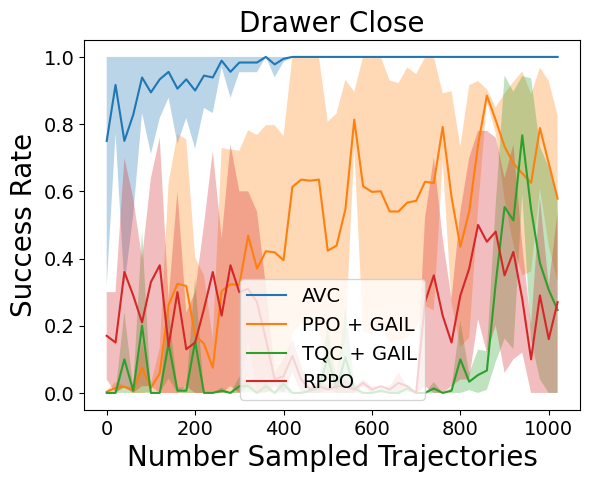
\includegraphics[width=\textwidth]{images/0/Drawer Close.png}
      \caption{Drawer Close environment.}
      \label{fig:plot1}
    \end{subfigure}
    \caption{No expert demonstrations were provided. 
    The x-axis shows the number of sampled environment epsiodes, each with 100 steps. One initial observation and a sparse reward signal at the end of each episode was provided.}
    \label{fig:fourplots}
\end{figure}

\subsetion{Reinforcement Learning}
In this section we analyze the performance of our algorithm on a selection of (4) Meta World tasks, with varying degree of expert demonstrations

4: Reach PickPlcae, Push, Windowopen 

1: Reach with only one example
-with planner without planner
-compare optimized vs. non optimized
-show how planner and actions change the trj. differently

0: Drawer Close with 0 examples
-compare optimized vs. non optimized
We chose these setups, as they demonstrate the abilities of AC.

